\documentclass{article}
\bibliographystyle{apalike}
\usepackage{natbib}
\usepackage{a4}[]
\usepackage{graphicx}
\usepackage{booktabs}
\usepackage[polish, english]{babel}
\addto\captionspolish{%
	\renewcommand{\tablename}%
	{Table}%
}

\addto\captionspolish{%
	\renewcommand{\figurename}%
	{Figure}%
}


\usepackage[T1]{fontenc}
\usepackage[utf8]{inputenc}
\usepackage{longtable}
\usepackage[a4paper,%
left=1in,right=1in,top=1in,bottom=1in,%
footskip=.25in]{geometry}
\usepackage{placeins}
\makeatletter
\setlength{\@fptop}{0pt}
\makeatother

\author{1632704}
\title{%
	The Dynamics of Political Polarization on Polish Twitter \\
	\large Under the supervision of Prof. Lukasz Walasek}


\begin{document}
	
	\maketitle
	
	
	\begin{abstract}
		
	The topic of political polarization in social networks has received significant attention throughout the last decade, however, little is still known about the temporal dynamics of this phenomenon, especially during periods punctuated by politically salient events, such as elections and nationwide crises. This paper analyzes the data gathered between February and July 2020, from a sample of Twitter users in Poland clustered around elites from two opposing parties. The duration of the study coincided with the run-up to the presidential elections and the outbreak of the COVID-19 pandemic. The partisanship estimator developed by Gentzkow, Shapiro and Taddy applied to the data allowed to identify a significant growth in polarization throughout the observed period, driven primarily by discussions related to public health, presidential candidates and the clash between conservative and progressive values. The findings support usefulness of the partisanship estimator for analyzing speech polarization in languages other than English, show the relevance of the cultural backlash hypothesis in explaining public opinion differences in contemporary Western and cast doubt on accounts of ideological divergence in nations faced by collective threats. \footnote{The Python code used to conduct the analysis can be found at https://github.com/piotrbogdanski/twitter}
	
	
	\end{abstract}

	\section*{Introduction}
		
	Political polarization has received increasing scholarly attention throughout recent decades \citep{lukianoff2018, tucker2018, sunstein2018}.  The growing availability of the Internet and the associated spread of social media platforms is closely tied to this phenomenon, however its impact has been widely contested. On the one hand, it is argued social media facilitate the emergence of so-called “echo-chambers', closed environments in which people encounter mostly views and information consistent with their beliefs, leading to an increasingly polarized society \citep{prior2007}. Through its very nature, social media makes group identity more salient and provides its users with a sense of anonymity - both of these characteristics were speculated to promote polarization in the past \citep{sunstein2002}. Moreover, concerns have been raised about the so-called ‘filter bubble’, a term describing the impact of the personalized suggestion algorithms used by most social media platforms, which can reinforce the exposure to belief-contingent content \citep{pariser2009}. However, the magnitude of the algorithms’ effect appears to be smaller in comparison with users’ deliberate choices \citep{bakshy2015}. On the other hand, some of the existing literature points at the opposite role of the modern means of communication - the analysis of the following-follower patterns of connection has shown that social media users are at least partly exposed to diversified information, and, as a result, engagement with social media is likely to reduce political polarization \citep{barbera2015_2, barbera2015_1}. Furthermore, some previous research has suggested that the extent of actual polarization has often been overestimated \citep{westfall2015}. Nevertheless, mere information exposure is likely to be insufficient for opinion forming, as the latter requires repeated interactions and is likely to be deeply affected by the homophily of social networks \citep[][pp. 192]{jackson2020}. Previous work shows that selective exposure is significantly greater in terms of content-sharing than follower\-followee relationships \citep{ogawaetal2013}. As a result, it is likely that polarization, understood as the divergence between views expressed by the ideologically opposed users, can remain high, despite the present level of cross-cutting information exposure.   
	
	This paper builds upon the previous findings and utilizes homophily of partisan social networks as a means to identify the relevant populations of partisan users. It attempts to disentangle the dynamics of ideological differences exhibited by their language in online conversations and to assess the impact of potentially polarizing events on their behaviour.
	
	The nature of the Polish political system makes it an interesting case study of political polarization. Despite being a multi-party democracy with proportional representation, for the past 15 years, Poland has exhibited largely bipartisan tendencies, with two major parties the liberal Civic Coalition (PO) and conservative Law and Justice (PiS) capturing the majority of the electorate, which was perfectly exemplified by the first round of the 2020 presidential elections, in which their candidates have captured more than 73\% of the total vote count, with the second round won by PiS’s candidate by a narrow margin of 51-49. The sharp partisan differences among the Polish elites can be traced back to the split within former anti-communist opposition which occurred during the early years of Poland’s transformation \citep{baylis2012}. 
	
	Analysis of survey data shows that these divides are reflected in the Polish electorate and that partisans are deeply polarized \citep{gorska2019}, at least in the sense of affective polarization, i.e. the strength of negative feelings towards the opposing party \citep{iyengar2012}. More importantly, there appears to be a degree of asymmetry in the strength of negative feelings, as the opposition supporters tend to dehumanize their counterparts more and express less trust towards them than the opposite. Those who side with the government also report more frequent interactions with their opponents, which appears to mitigate lack of trust and negative feelings towards them, which are less pronounced than in the opposite direction \citep{gorska2019}. This asymmetry runs contrary to the previous findings from other countries, which have shown a higher tendency amongst liberals to engage in cross-ideological communication \citep{barbera2015_2}.
	
	With respect to social media, research by Matuszewski and Szabó has found that Polish Twitter users are considerably biased politically, however, at the same time, users in all political clusters appear exposed to news from diversified sources, which mitigates the strength of partisanship-based echo chambers \citep{matuszewski2019}. The same pattern was present in political discussions on Facebook - while users are significantly polarized in terms of the liking activity and the sentiment of their comments is in line with their partisan attachments, the news sources cited by users are diversified \citep{matuszewski2018}.
	
	The period of the following study coincided with the run-up to the aforementioned presidential elections, an event that has serious implications for the study of political polarization. It has been argued that even under the assumption of voter rationality, polarized information environments can lead to irrational decisions undertaken by voters \citep{bernhardt2008}. This implies that the growth of political polarization is potentially detrimental for the democratic process itself. Fishkin has famously asserted that “deliberative democracy”, with a diversity of viewpoints and equal access to accurate information is an important precondition for a just political system \citep{fishkin2009}. Political polarization as such undermines the very prerequisites of this model \citep{sunstein2002}. At the same time, research shows that social media users tend to be strongly polarized prior to the “celebration of democracy” embodied by the elections \citep{conover2011, grover2019}. In conjunction, these conclusions from past work may hint at a possible vicious cycle of polarization, in which the democratic procedures coincide with growing polarization, which ends up undermining their effectiveness. Such a process is particularly problematic in the age of illiberal democracies, which threatens to affect post-communist countries in particular \citep{zakaria1997}.
	
	One of the most significant events that were likely to have shaped the partisan debate over the period of the study was the COVID-19 crisis, the largest global pandemic since the Spanish Flu of 1918, which claimed the lives of thousands of people and disrupted the day-to-day functioning of millions around the world. The impact of such events on political polarization remains largely undescribed, due to their extremely rare nature. Previous work on the Ebola crisis in the US has found that social networks play a polarizing role in the discussion of the public policy response to such health crises and reduce partisans’ propensity to support decisions guided by scientific evidence \citep{elmedni2016}. Responses to significant military crises, such as the Iraqi War of 2003 have also been found to be differentiated along party lines, with the main role played by selective exposure to partisan news outlets \citep{jacobson2010}. Similar tendencies have emerged during the COVID pandemic, as exposure to different news sources was found to be predictive of people’s compliance with social distancing measures imposed in the US during the pandemic \citep{bursztyn2020}. 
	
	The theoretical predictions regarding the relationship between diseases and political behaviour are mixed. On the one hand, research related to the so-called “behavioural immune system” has shown that salience of epidemiological risks is likely to enhance people’s xenophobic attitudes and in-group favouritism, especially when the out-group comes from an unfamiliar cultural background \citep{faulkner2004, kim2016}. The topic of refugee rights was highly polarizing in Polish political debate during the 2015 parliamentary campaign \citep{matuszewski2018}, however, was largely absent since the decline of the Mediterranean migration crisis. Furthermore, nationwide crises provide an opportunity for the government supporters to endorse actions undertaken to mitigate its results, while the opposition is expected to capitalize on any perceived failures, especially during the build-up to elections. 
	
	On the other hand, previous findings show that crises tend to evoke favourable attitudes towards the incumbent, a phenomenon known as the ‘rally-around-the-flag effect’. Muller has argued that this process arises when the said crisis is an international event that involves the country directly and is salient in the public discussion, which fits the circumstances of the COVID-19 crisis well \citet{mueller1970}. Evidence from Denmark shows that an increase in trust in the government and public institutions was observed since the introduction of the COVID lockdown, in accordance with previous findings \citet{baekgaard2020}. Moreover, a decrease in ideological differences during periods of collective threat has been documented in the past and was mostly attributed to a “conservative shift” observed amongst the liberals \citep{bonanno2006, vandevyver2016}. This is consistent with the notion of “authoritarian reflex”, which is likely to be triggered by exposure to perceived physical threats \citet{norris2019}. At the same time, the nationwide economic lockdown imposed due to the pandemic has invoked fears of economic recession. It’s been long found that fears of economic crisis reduce the governmental support \citep{lewisbeck2000}, and, more importantly, that adverse economic conditions, albeit experienced rather than anticipated, make individuals more likely to support extremist politics and tend to ideological realignment \citep{autor2016}.
	
	Finally, the COVID pandemic had serious country-specific implications in Poland, as it spurred a major debate related to postponing the upcoming presidential elections planned for 10th of May 2020. Initially, the government has pushed to keep the original date and to rely on postal voting, which led to accusations of fraud attempts, likely endangerment of public health and calls for boycotting the ballot from the opposition parties. The elections were eventually postponed to the 12th and 28th of July, first and second round respectively.
	
	As outlined above, previous work on polarization yielded definitive answers neither with respect to the role of social media, nor its relationship with nationwide crises. This paper uses the data collected from Polish Twitter users in the first half of 2020 analyse polarization during the build-up to the election date and shed light onto those questions. Firstly, the partisanship estimator \citep{gentzkow2019} based on Bag-of-Words representation of partisan tweets were used to examine the extent of language polarization. Secondly, a topic analysis was conducted using Latent Dirichlet Allocation to identify the most relevant topics discussed by partisans over the period of the study. Thirdly, partisanship was re-estimated within these topics, to evaluate topic-specific polarization. Finally, party-specific phrases in each of the topics were examined to gain a direct insight into differences between Polish partisans.
	
	\section*{Data Collection}
	
	The data was collected between the 23rd of February and 15th of July using Twitter's open API from a sample of 10000 users, with half of them categorized as opposition partisans and the other half as government supporters. To approximate the users’ party allegiance, 10 profiles of highly followed Twitter politicians affiliated with the ruling party and the main opposition party were selected (see Table \ref{tab:seed_profiles}). These accounts were used as “seed profiles” to obtain a complete list of their followers. Previous research has shown that the homophily of a users’ network is an effective method of determining her political preferences \citep{volkova2014}. Based on this assumption, profiles that follow more than 5 politicians from one source and less than 5 to the other were filtered out. The later constraint was imposed to ensure that users with high interest in politics or bot profiles who follow profiles of major politicians regardless of their party affiliation are not included in the final sample. The resulting set consisted of 26465 opposition and 35422 government profiles. Due to the data load, 5000 users active at least once in February were selected from each group. It’s important to note that the main limitation of the described data gathering process is the implicit assumption of a dichotomous structure of users’ political preferences, despite supporters of smaller political parties who also take part in the online discussions. However, as mentioned earlier, the bulk of the Polish electorate is divided between PO and PiS. Previous findings also show that supporters of other parties tend to be positive with respect to members of political clusters that are close on the left-right political continuum \citep{matuszewski2018}. Such framing is also in line with the nature of presidential elections in a majoritarian system, where the final outcome usually depends on the 2 round contest between the two main candidates.
	
	In total, 9 484 966 tweets were collected. Each message was lemmatized using Stanza Polish lemmatizer and Part-of-Speech tagger \citep{qi2020}. The PyEnchant Python library was used to recognize Polish words in order to compute the proportion of Polish lemmas in each of the messages. Users whose average proportion of Polish tokens per tweet was below 0.4 were removed entirely from the analysis. Furthermore, messages with less than half of Polish lemmas were also not considered. Additionally, one user who posted a suspiciously large number of messages per day was removed from the sample. The final sample consisted of 9 116 072 tweets from 9713 (4870 government, 4843 opposition) users.
	
	
	\section*{Tweet Partisanship Over Time}
	
	\subsection*{Method}
	
	To estimate the changes in polarization within the sample over time, the leave-out estimator of partisanship developed by \citet*{gentzkow2019} was applied The model was previously successfully used as a tool to examine evaluation on Twitter \citep{demszky2019}. 
	
	The estimator describes the polarization of a given speech as the posterior probability that an observer with a neutral prior assigns the speaker to his right party based on a randomly selected word from the speech. The observer is assumed to know the underlying speech-generating process of both parties, which follows a multinomial probability distribution with specific probabilities assigned to each of the phrases. In other words, the polarization score varying between 0.5 and 1.0 can be interpreted as the probability of assigning a user to his party allegiance correctly based on a randomly selected phrase from his Tweets. Additionally, the leave-out estimator does not include the phrase counts used by each individual speaker to obtain the total counts for his or her party, which reduces the estimation bias. Formally, the partisanship is estimated by computing: 
	
	\begin{equation}
		\hat{\pi}_{t}^{LO} = \frac{1}{2} \frac{1}{|R_{t}|} \sum_{i \in R_{t}} \hat{q}_{i,t}  \cdot \hat{p}_{-i,t} +  \frac{1}{2} \frac{1}{|D_{t}|} \sum_{i \in D_{t}} \hat{q}_{i,t}  \cdot (1 - \hat{p}_{-i,t})\\
	\end{equation}

	\centerline{where, }
	
	\begin{equation}
			\hat{p}_{-i,t} = \hat{q}_{-i,t}^{R} / (\hat{q}_{-i,t}^{R} + \hat{q}_{-,it}^{D})
	\end{equation}
	
	\centerline{describes the probability of an observer with a neutral prior}
	\centerline{assigning a speaker to government based only on a given phrase and}
	
	\begin{equation}
		\hat{q}_{i,t} = c_{i,t} / m_{i,t}
	\end{equation}
	 \centerline{are the phrase frequencies for speaker $i$ at time $t$}
	 
	 \bigskip
	
	The phrase counts used to obtain the party-specific speech-generating model were obtained individually for each day in the analysis. While the choice of day as a timestep for measurement is somewhat arbitrary, re-estimating the polarization using weekly pooled data did not alter the conclusions of the analysis. To further ensure the robustness of the results, partisanship was also estimated based on a moving window of 7 days surrounding the day for which the estimate was computed, using unique tweets only (i.e. including retweets, but only once for every 7-day window containing the estimate, as well as for Tweets with the number of tokens above the median within a given day, which yielded comparable results (see Figure \ref{fig:polarization_moving_window}). The model was fitted for each day on a collection of unigrams and bigrams obtained after lemmatization and stopword removal, which were used by the users at least 40 times within the day, which are the same thresholds as the ones used by the analysis by \citet{demszky2019}. The confidence intervals were computed by bootstrapping 100 samples of 10\% of the users for each time point and randomly assigning them to political parties \citep{politis2001, gentzkow2019}. In order to verify whether any degree of political polarization was present, a randomization test was performed, in which each user was randomly assigned to a party and the estimates were recomputed along with the confidence intervals.
	
	\clearpage
	
	\subsection*{Results}
	
	\begin{figure}[h!]
		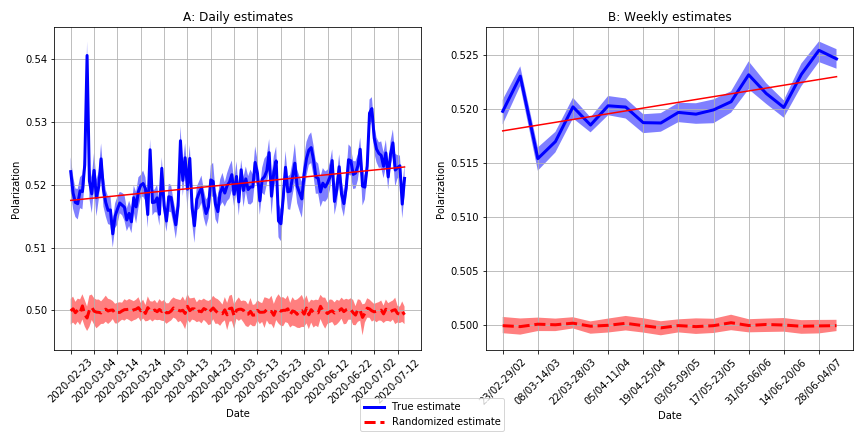
\includegraphics[width=\columnwidth]{figures/polarization_overall.png}
		\caption{Estimates of partisanship over time}
		\label{fig:overall}
	\end{figure}

	The results of the analysis can be seen in Figure \ref{fig:overall}. Panel A presents the daily estimates, while Panel B shows the partisanship computed on weekly level estimates of partisanship. It can be seen that the polarization across the entire 6 month period preceding the elections was significantly greater than due to random assignment. The randomization estimates oscillate around 0.5 with roughly 0.02 margin of error, meaning that when parties are assigned at random each there’s an equal probability of assigning each user to his or her party. The true estimates, on the other hand, vary in the range between 0.518 and 0.542 with confidence intervals never reaching the threshold of 0.5, which implies that throughout the entire period of the analysis, a random observer would be more likely to assign a user to his true party after seeing a random phrase from his message. 
	
	Secondly, both daily and weekly estimates have statistically significant positive trends ($\beta = .0000378$, $p < .001$ and $\beta = .000265$, $p < 0.001$ respectively), while their randomized equivalents aren’t different from 0. The effect size may appear small, however, over the 150 days of the analysis, this translates to an increase in partisanship by 0.5\%. The time-series constituted by the day-level estimates is also significantly autocorrelated in the first 3 lags (see Figure \ref{fig:autocorrelation_overall}), suggesting that the polarization dynamics over time exhibit the properties of an autoregressive process. Since the data spans the entire run-up to the presidential elections, which took place on the 12th of July 2020, this trend indicates that the closer to the elections, the larger were the differences between the partisans. The next section focuses on decomposing this trend into the topics discussed by partisans on Twitter.
	
	\clearpage
	
	\section*{Topic analysis}
	
	\subsection*{Method}
	
	In order to evaluate the relative importance of different issues deliberated in Twitter discussions, the topics were identified using the LDA unsupervised model \citep{pritchard2000, blei2003}. The intuition behind Latent Dirichlet Allocation, a common technique used for topic modelling, is that it attempts to find a predefined number of topics that maximize the likelihood of each topic occurring in a given document and the likelihood of each token occurring in a given topic within the corpus. To train the model, the MALLET implementation of LDA \citep{mccallum2002} was used through the Gensim API. MALLET utilizes an efficient method for optimizing the model’s hyperparameters. Due to computational limitations, the models were fitted on a random sample of 10\% of the data, stratified by each Tweets party label and date and including only Tweets with unique lemmas within a given day and party. A total of 521514 observations were used to train the models. The number of topics was chosen through a grid search (see Figure \ref{fig:coherence_grid}) in order to maximize the coherence score of the resulting topics, a method which evaluates a topic model by applying a 4-step pipeline of topic segmentation, probability estimation, computing a confirmation measure (pointwise mutual information) and aggregating the measure over the dataset \citep{roder2015}. The best model identified 28 topics within the discussion and the resulting topic assignment reached the coherence score of 0.526 on the training set. Since many of the messages are likely to consist of a mixture of multiple topics, an approach suggested by \citet{demszky2019} was utilized to filter out undetermined Tweets - all observations with a ratio of the first and second closest topic smaller than the 0.2 quantile of the distributions of such ratios in the training set were filtered out as “difficult to identify” and not included in the analysis of within-topic polarization.
	
	\subsection*{Results}
	
	\begin{figure}[!ht]
		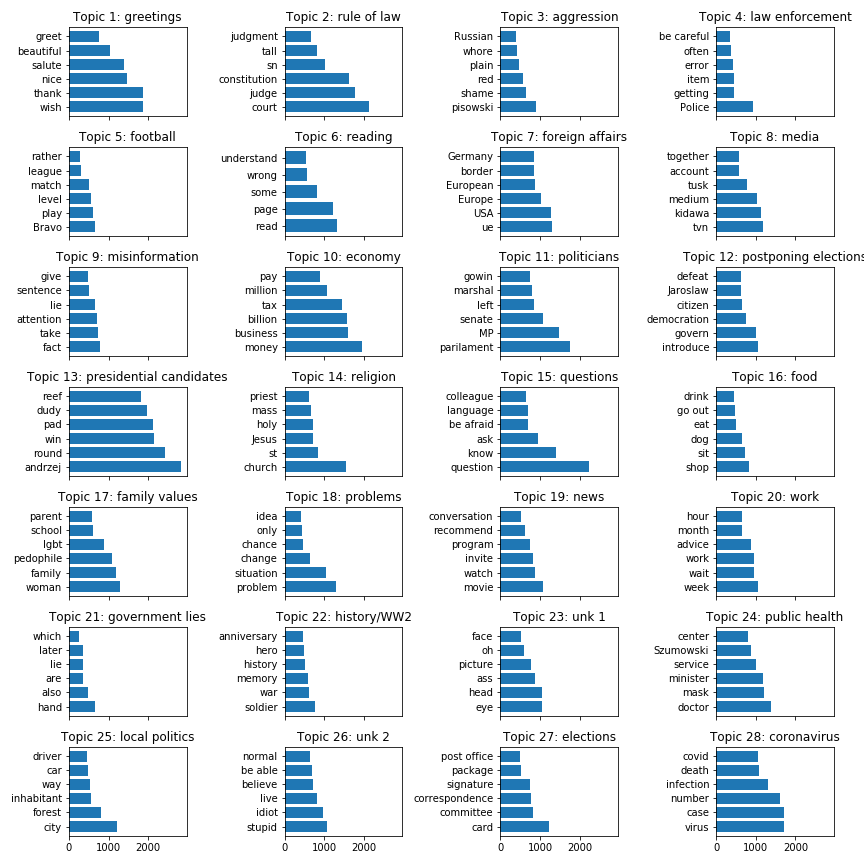
\includegraphics[width=\columnwidth]{figures/topic_tokens_en.png}
		\caption{Most representative tokens in each of the 28 topics identified by the best LDA.}
		\label{fig:topic_tokens}
	\end{figure}

	The content of the topic is summarized by Figure \ref{fig:topic_tokens}, which presents the translations of the most common unique tokens in each of the topics, meaning that these tokens have not occurred in the top 50 tokens of every other topic in the corpora. Such a summary is more meaningful, as it discards some words that occurred frequently in multiple topics due to the very nature of the Twitter discussions common amongst the sample, such as “Poland” or the names of political parties. The unfiltered most common tokens can be found in the Appendix. As expected, topics related to the COVID pandemic - the pandemic itself (most frequent tokens ‘virus’, ‘case’, ‘number’, ‘infection’) and public health response (‘‘doctor’, ‘mask’, ‘minister’, ‘service’), as well as presidential elections - the administrative approach to voting necessitated by the crisis (‘card’ [ballot], ‘commission’, ‘correspondence’) and presidential candidates (‘andrzej’, ‘round’, ‘win’) were present in many of the Tweets. Other prominent political topics in Polish political discussions, such as the economy (‘money’, ‘business’, ‘billion’), religion (‘church’, ‘saint’, ‘jesus’), the judiciary reform (‘court’, ‘judge’, ‘constitution’), foreign affairs (‘EU’, ‘USA’, ‘Europe’), media (‘tvn’ [main liberal news outlet], ‘Kidawa’ [first opposition presidential candidate], ‘media’), family values and sexual minorities (‘woman’, ‘family’, ‘paedophile’, ‘lgbt’), politically charged aggression (‘pisowski’ [adjective from PiS], ‘shame’, ‘red’) and WWII (‘soldier’, ‘war’, ‘memory’). The model has also identified Tweet clusters less related to politics, including football (‘bravo’, ‘play’, ‘level’, match) or common civilities (‘wish’, ‘thank’, ‘nice’). Some of the topics were difficult to identify (e.g. topic 23, topic 26).
	
	\clearpage
	
	Figure \ref{fig:topics_time} provides an overview of the temporal distribution of the selected relevant topics (the distribution for all can be found in the Appendix). Most notably, it can be seen that the specific topic related to the COVID pandemic was mainly popular at the beginning of the European outbreak, mainly in March and early April. Since the beginning of May, it drastically reduced its share of the online conversations, giving room to the emergent discussions related to the upcoming elections. Notably, the topic related to family values increased in the share before the elections, which was confirmed in the media debate started by accusations thrown by PiS’s presidential candidate, Andrzej Duda, against the “LGBT ideology” \citep{financial_times2020}.
	
	\begin{figure}[!h]
		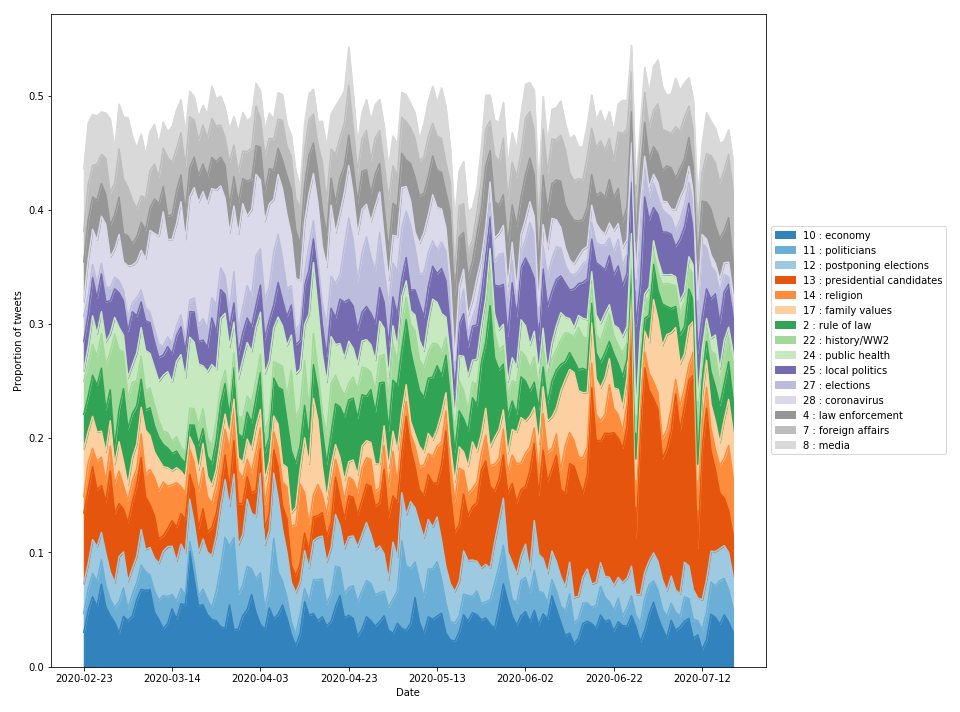
\includegraphics[width=1.1\columnwidth]{figures/temp_dist.png}
		\caption{Proportion of selected topics in Twitter discussions over time of the study.}
		\label{fig:topics_time}
	\end{figure}

	Finally, the violin plot in Figure \ref{fig:topic_proba} depicts the log-odds of being a government partisan given Tweeting on a certain topic. Since members of the two groups differ significantly in terms of their ideology, it was expected that differences will be present in their topic preferences. The results seem to suggest that some degree of between-topic polarization (discussed further in the following section) were present. In particular, government supporters appeared more likely to Tweet about religion and history, while the opposition supporters were more likely to Tweet about elections, postponing them, the rule of law and the economy. Government users, on the other hand, focused more on topics related to religion and history.
	
	\begin{figure}
		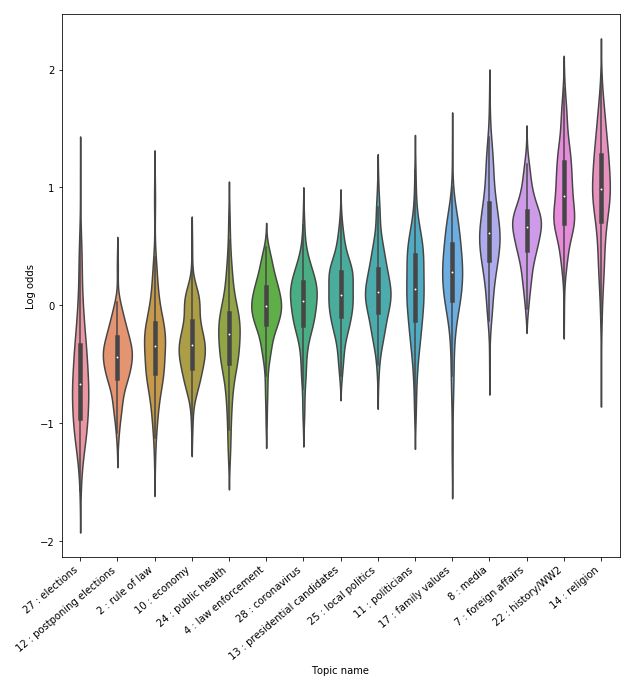
\includegraphics[width=\columnwidth]{figures/topic_proba.png}
		\caption{Log odds of being a government follower given selected topic.}
		\label{fig:topic_proba}
	\end{figure}
	

	
	\clearpage
	
	
	\section*{Topic polarization}
	
	\subsection*{Method}
	
	Following Gentzkow’s methodology, the obtained topics were used to decompose partisanship into its between-topic and within-topic components. Between-topic partisanship refers to the differences in users Tweets attributable to the choice of different topics and is estimated by computing the posterior probability of a neutral observer assigning the right party to the speaker knowing only the topic of the Tweet. Within-topic partisanship is simply the weighted average of partisanship estimated only for tweets within a particular topic. This was estimated in the same way as overall partisanship, but using only tweets that refer to each topic identified by the LDA model. 
	
	\subsection*{Results}
	
	\begin{figure}[!h]
	
		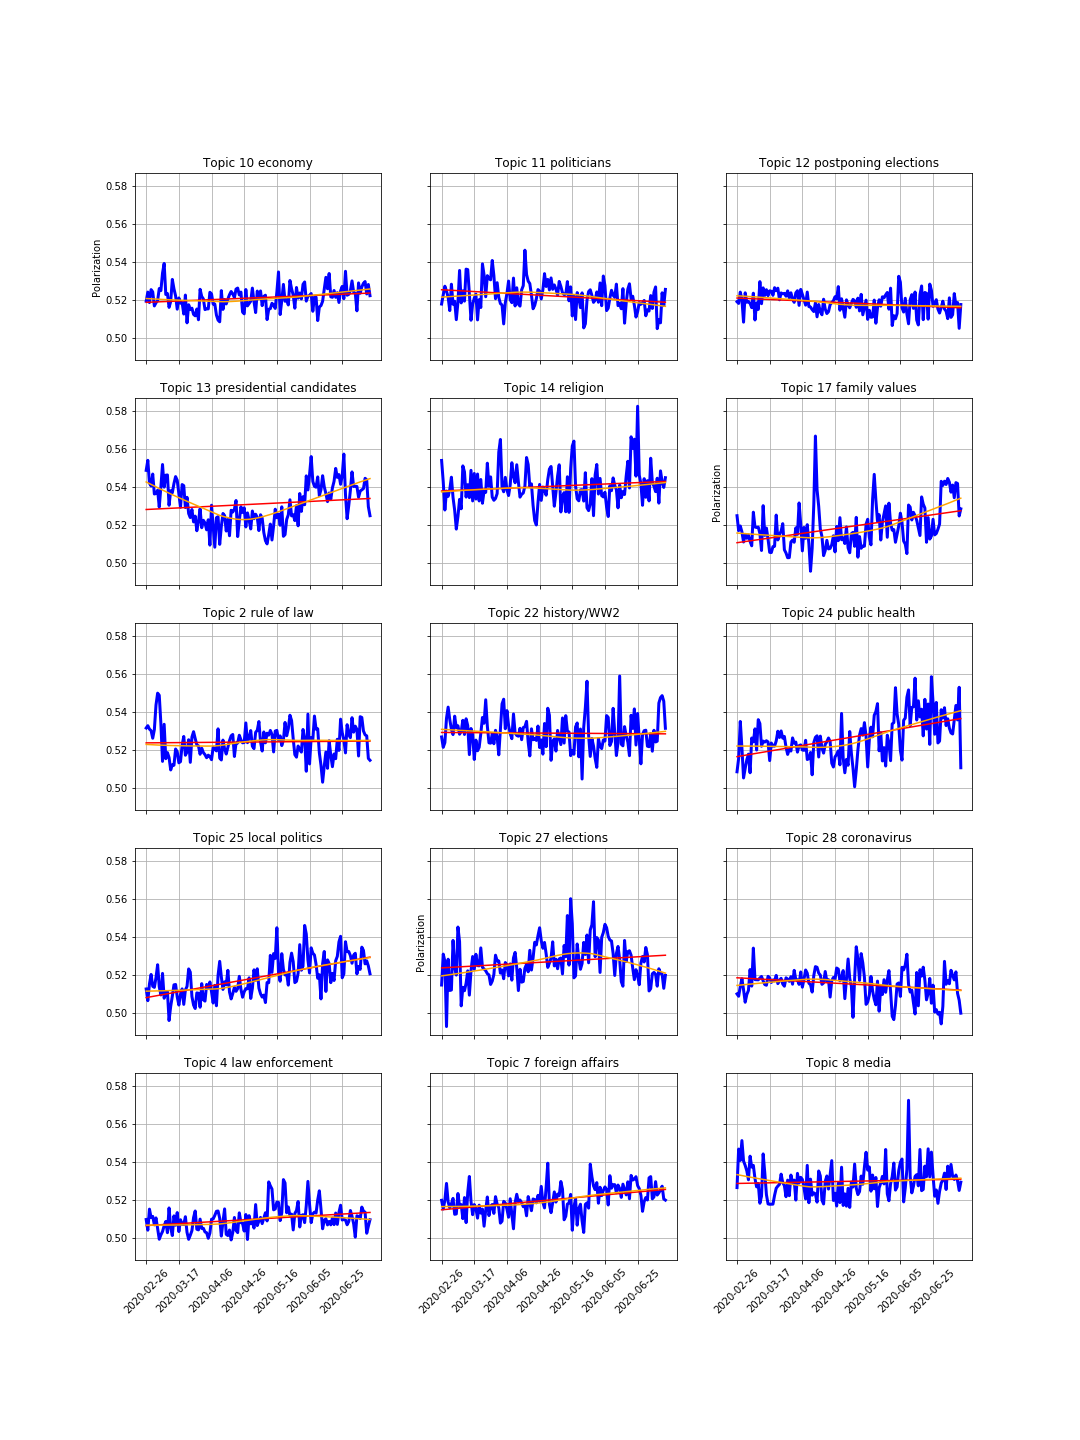
\includegraphics[width=\columnwidth]{figures/polarization_topics.png}
		\caption{Polarization estimates over time within selected topics. Polarization for all 28 topics can be found in Figure \ref{fig:polarization_topics_all}}
		\label{fig:partisanship_topics}
	
	\end{figure}

	Figure \ref{fig:partisanship_topics} presents the variation of polarization within each of the topics across time. The changes over time are most pronounced in the topic related to presidential candidates. It can be seen that in late February, which coincided with the commencement of the major candidates presidential campaigns, the level of polarization within that topic was at its highest level. With the onset of the COVID pandemic, polarization within that topic has sharply declined, however the overall polarization did not. This can be attributed to polarization in other topics, primarily the more general topic related to the elections and the legitimacy of postal voting. The polarization within this topic decreased when elections were closer and so did the topic’s popularity (Figure \ref{fig:topics_time}). At the same time, growing polarization could be observed in other topics, most notably, presidential candidates, public health and family values, which contributed to the overall pre-election growth in polarization. The topic related to local politics was also a source of differences between Twitter partisans, which is likely related to the fact that the liberals’ party presidential candidate was the mayor of Poland’s capital, Warsaw. The trends are further summarized by Figure \ref{fig:partisanship_topics_coef}, which presents the OLS estimates of the slope for each of each series. Note that while the linear slope was not significant for presidential candidates and elections, it has shown statistical significance for quadratic coefficients (both at p < 0.001). \footnote{For the exact estimates, see Figure \ref{fig:partisanship_topics_coef_quadratic} and Tables \ref{tab:polarization_topics_ols} and \ref{tab:polarization_topics_ols_quadratic}}
	
	\begin{figure}[!h]
		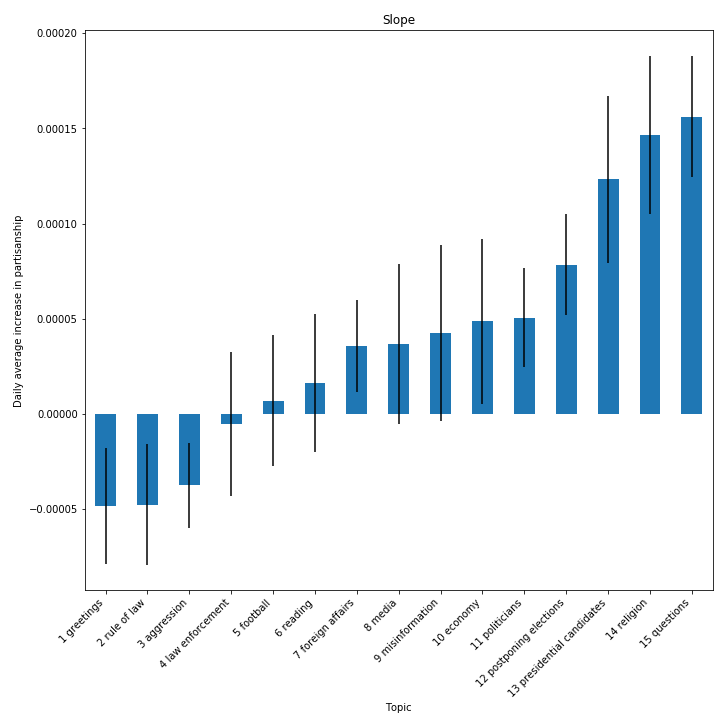
\includegraphics[width=\columnwidth]{figures/partisanship_topics_coef}
		\caption{Slopes of OLS fits for trend in selected topics.}
		\label{fig:partisanship_topics_coef}
	\end{figure}

	The break-down of partisanship into its within-topic and between-topic components is shown in Figure \ref{fig:partisanship_within_between}. It can be clearly seen that throughout the run-up to the elections, polarization between topics has remained constant or even decreased, which implies that the topics chosen by partisans were relatively homogenous across groups. At the same time, the average of polarization within all the identified topics has been growing and follows a pattern very similar to the overall polarization. In fact, the correlation between the within and overall estimates over the period of the study was 0.719 as compared to more moderate value of 0.267 between the overall and between estimates. This seems to suggest that the growth in partisanship of views expressed by Polish Twitter users was mainly driven by different ways of discussing the same topics, rather than mere differences in topics that they touched upon.
	
	\begin{figure}[!h]
		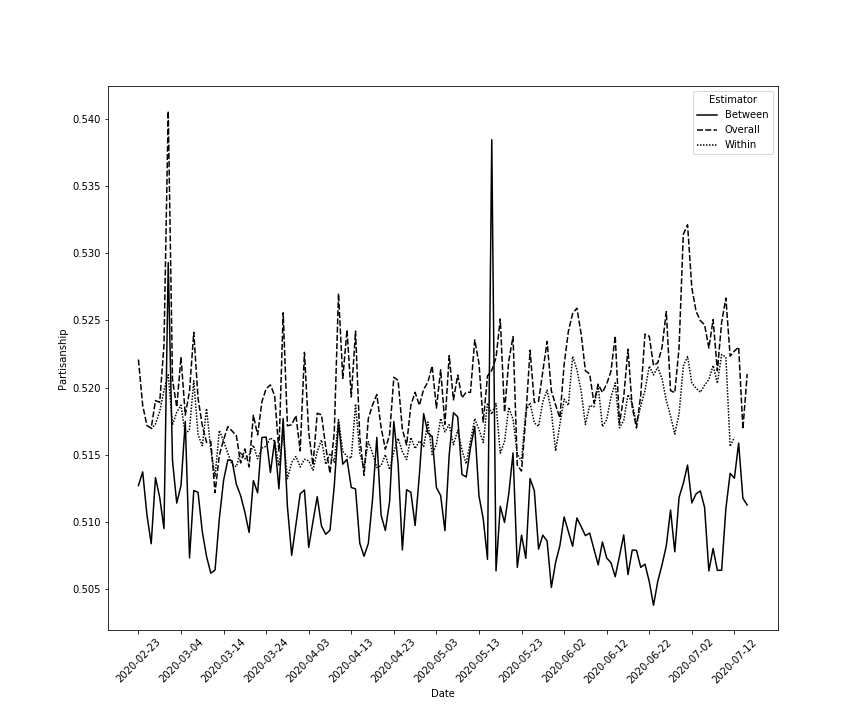
\includegraphics[width=\columnwidth]{figures/partisanship_within_between.png}
		\caption{Comparison of within-topic and between-topic estimates of partisanship with overall partisanship over time.}
		\label{fig:partisanship_within_between}
	\end{figure}

	\clearpage
	
	\section*{Phrase partisanship}
	
	\subsection*{Method}
	
	The final step of the analysis was aimed at gaining a direct insight into the framing used by supporters of each of the parties with respect to the polarizing topics. To do that, phrase polarization for each day and topic was approximated simply by probability of choosing a given phrase to discuss this topic given users’ party, again using unigrams and bigrams that occurred at least 40 times during a given day. This reflects how much was a word mentioned by partisans of one of the sides, comparatively to the other. Then, the average of each probability weighted by the number a phrase has occurred on each day was computed, to provide a final estimate of the probability of phrase selection.\footnote{The original, untranslated Polish lemmas and English translations of lemmas for all 28 topics can be found in Tables \ref{tab:party_phrases_pol_full} and \ref{tab:party_phrases_en_full} respectively}
	
	\subsection*{Results}
	
	\begin{longtable}{p{2cm}p{6cm}p{6cm}}
		\toprule
		topic label &                                                                                                                                                                opposition phrases &                                                                                                                                                                               government phrases \\
		\midrule
		rule of law &                                 pisowski [governing party], Kaczynski [PiS leader], PiS [governing party], ribs, Duda [incumbent president], legal basis, krs, equal, mode, party &                                                                                                     caste, reform, gersdorf, opposition, tsue, insert, end, extraordinary, Pole, president of sn \\
		law enforcement &                                                            fog, shadow, sharp, Duda [incumbent president], PiS [governing party], authority, country, police officer, feel, right &                                                     opposition, world, Trzaskowski [opposition presidential candidate, Mayor of Warsaw], coronavirus, Pole, to stop, one, use, similar, behavior \\
		foreign affairs &                                                                         community, PiS [governing party], Morawiecki, Belarus, European union, trump, union, American, live, open &                                                                                                independent pl, independent, defenka, Berlin, opposition, tusk, Brussels, German, security, Spain \\
		media &                                                            excursion, pi, PiS [governing party], affair, public, strong together, propaganda, strong, tvp, Kaczynski [PiS leader] &  gw [liberal newspaper], nitras [opposition MP], sok burak [online opposition platform], burak, Budka [opposition leader], sok [online opposition platform], platforms, fake news, Nov, platform \\
		economy &                              pisowski [governing party], Szumowski [Health Minister], Kaczynski [PiS leader], bagpipe, pi, Morawiecki, coal, tvp, PiS [governing party], free tax &                                                              ofe, psl, tusk, Trzaskowski [opposition presidential candidate, Mayor of Warsaw], Warsaw, pit, retirement age, retirement, age, gas \\
		politicians &                                          Kaczynski [PiS leader], electoral, left, Witek [Speaker of the Parliament], correction, vote, right, reject, PiS [governing party], sign &                                      total opposition, total, township, confederation, Bosak, town marshal, sld, civil, Trzaskowski [opposition presidential candidate, Mayor of Warsaw], Poland \\
		postponing elections &   pisowski [governing party], maintain, pi, Kaczynski [PiS leader], PiS [governing party], Morawiecki, corpse, Duda [incumbent president], government pis [governing party], hand &                                                 psl, total, tusk, opposition, chaos, Trzaskowski [opposition presidential candidate, Mayor of Warsaw], Polish, take over, go, state of emergency \\
		presidential candidates &       PAD out of palace, padz, President of Trzaskowski [opposition presidential candidate, Mayor of Warsaw], palace, wkk, powerful, Biedron, Kaczynski [PiS leader], left, enter &         double, Duda president [incumbent president], duda andrzej [incumbent president], knowmore, president andrzej, case, Polish, President Duda [incumbent president], plan, booty elections \\
		religion &                                                                                                 religion, divine, bishop, Catholic, miracle, priest, Catholic, go, church, Polish &                                                                                                              bless god, happiness, God bless you, mercy, pay, St. John, mass, st, Paul ii, thank \\
		family values &                                                          Duda [incumbent president], pedophile, PiS [governing party], victim, violence, President, person, Polish, to, education &                                                               abortion, Trzaskowski [opposition presidential candidate, Mayor of Warsaw], ideology, man, black, schools, mother, lgbt, life, old \\
		history/WW2 &  PiS [governing party], Smolensk [location of 2010 presidential plane crash], Kaczynski [PiS leader], a disaster, grave, good, power, Duda [incumbent president], man, each other &                                                                                                                    last, soviet, Communist, late, stanislaw, German, john, ps, Communist, German \\
		public health &                               PiS [governing party], test, elections, health ministry, Duda [incumbent president], prepare, protection measure, health protection, ministry, lack &                                                                                           operation, Owsiak [liberal health activist], save, thank, beg, rt, thousand, to support, help, support \\
		local politics &                                                                                   electric, PiS [governing party], region, animal, Wroclaw, drought, car, Szczecin, climate, flat &                                                         town hall, Czajka [malfunctioning sewage treatment plant in Warsaw], zone, read, Warsaw, Vistula, capital, gdańsk, Warsaw, Vistula river \\
		elections &                          sasin [Interior Minister], sasina [Interior Minister], Kaczynski [PiS leader], print, Jack, print, organize, PiS [governing party], voting card, package &                                                                                  envelope, opposition, promise, collect a signature, station, polling station, take place, collect, term, poster \\
		coronavirus &         PiS [governing party], pi, Duda [incumbent president], number of test, elections, Szumowski [Health Minister], sanepid [CDC equivalent], do the test, to test, to perform &                                                                                            knowmore, voiv, Sweden, Spain, coronavirus sars, covid coronavirus, vaccines, flu, wuhan, coronavirus \\
		\bottomrule
		\caption{Top 10 most partisan lemmas for selected topics. Explanations of specific proper nouns in brackets.}
		\label{tab:phrases}
	\end{longtable}
	
	
	Table \ref{tab:phrases} presents the polarized phrases. The partisans seemed to have used dissimilar vocabulary to discuss the polarizing topics. In case of the coronavirus pandemic, the supporters of the opposition were mainly focused on testing, which corresponds to the debate on insufficient testing being conducted by the government. The government affiliated users, on the other hand, were much more likely to discuss the coronavirus location, vaccines, as well as its origin and other countries (Spain, Sweden, with China and Italy in the top 20 government-specific phrases). This seems to suggest that government partisans were likely to focus on the crisis outside, rather than inside of the country. Within the public health topic, opposition supporters focused on the medical staff and health protection, while their opponents discussed possible health support. In the discussion on elections, opposition partisans were mainly concerned with the postal voting ballots printed by the interior minister Sasin, while the government seemed to have mainly sided with organizing the May elections despite the pandemic. In the debate surrounding the candidates, supporters of each respective party mentioned their own candidate, with opposition also much more likely to mention secondary presidential candidates from other parties. The behaviour was also highly differentiated within the topic of the economy, where government partisans were most likely to mention the failures of the opposition government from before 2015, the topic which dominated their economic discussion prior to the 2015 parliamentary elections as well \citep{matuszewski2018}. Opposition, on the other hand, was more concerned with fears of the recession and public finance. In long-standing debates such as the judiciary reform or foreign affairs,  the partisans seemed to have followed the expected divisions, with government partisans focusing on issues related to the current judiciary system in the former and perceived enemies (Brussels, Berlin, Germany) in the later, while their counterparts discussed topics such as respect for the rule of law and european unity respectively. Finally, within the debate on family values, opposition users were more likely to reference sexual education and violence (presumably against the LGBT community), while government users referenced ‘ideology’ (following President Duda’s assertion on LGBT ideology \citep{financial_times2020}), mothers, children or abortion.
	
	\clearpage
	
	
	\section*{Discussion}
	
	The above analysis offers new insights into the dynamics of political polarization on social media. Firstly, it supports the the model proposed by Gentzkow, Shapiro and Taddy as a powerful technique for capturing partisan differences regardless of the language it is applied to. It also provides an external validation of the concept of homophily as basis for partisanship, as a sample of users selected solely on the basis of politicians they follow show significant differences in the language they use in their tweets. This confirms previous findings both in reference to Polish social media \citep{matuszewski2018, matuszewski2019} and social media in general \citep{volkova2014, demszky2019} . Secondly, as expected, the occurrence of significant political events appear to coincide with exacerbation of cross-partisan differences. This seems to be driven mainly by expressing opposed opinions with regard to the candidates, but was also significantly affected by the context of the current crisis. 
	
	The data also provides insights into the newly emerging question of the impact of the COVID crisis on public opinion dynamics. While polarization within the discussions about the pandemic has not shown noticeable trends over the period of the study, the topic has still divided the partisans and captured their attention for a significant period of time, driving it away from the typically discussed matters. Moreover, it indirectly fed into the pre-presidential debate, through the significantly polarizing topics of postponing the elections and the public health crisis. While nation-wide emergencies may lead many to ‘rally around the flag’, strongly opinionated users seem to be further divided and express significantly different opinions on the crisis response. This confirms previous accounts of the polarizing impact of social networks on crisis response \citep{elmedni2016, jacobson2010}. It is worth noting, however, that previous work has related these effects primarily to echo-chambers and selective news exposure. Neither of these seems to be the case within Polish partisan networks, as recent analysis has demonstrated that Polish users follow diversified news sources \citep{matuszewski2018}.
	
	Furthermore, the reported findings cast doubt on the previous accounts of “conservative shift” \citep{bonanno2006} invoked by collective threat, as no significant convergence of opinions has occurred since the beginning of the pandemic, neither on general level, nor within COVID-specific topics. This does not necessarily mean that the findings are entirely inconsistent with the “conservative shift” theory. Majority of research on that topic was conducted with respect to crises that were easily linked with a well-defined out-group, such as Muslims \citep{bonanno2006, vandevyver2016} or opponents in a civil conflict \citep{porat2019} and the resulting conservative shift was related to feelings of collective angst and strongly negative feelings towards the out-group. In the case of the COVID pandemic, no such out-group existed, therefore it is reasonable that collective angst presumably experienced by both groups would simply fuel their partisan identities. This is particularly true for the liberal opposition, as those responsible for the country’s public health are easy to blame for the perceived angst. It is important to stress that those conclusions should be treated with caution. The Polish data violates the ceteris paribus clause in which the conservative shift proposition should be evaluated, as the level of polarization was affected not only by the collective threat posed by the pandemic, but also by the presidential elections, a force expected to fuel divergence of opinions, which was confirmed by the data. While this is partially controlled for, as the coronavirus-specific topics were examined in isolation, it is impossible to rule out multitude of idiosyncratic interactions between those two factors. It is clear that once elections were closer they became more salient and captured the partisan attention, dwarfing the discussions related to the virus itself, both in terms of its popularity and its capacity to divide. Moreover, it is possible that a rightward shift of the ideological center of the discussion, with partisan divergence from the center still increasing. The results of the phrase analysis, however, render such interpretation unlikely.
	
	The second major theme in the analysis was the qualitative difference in interpretations of the main topics present in the public debates. Government partisans tended to focus on the crisis outside of the country’s borders and divert the attention to past issues, which was true both in case of coronavirus discussions and the economy, while opposition paid closer attention to the health and economic issues posed by the crisis. This is consistent with past research on partisan biases in perception of the political reality. According to \citet{bartels2002} the process of political learning is far from rational Bayesian updating, in which voters’ perceptions are expected to converge, especially if strong evidence is available. As already mentioned, prior research has shown that Polish partisans are exposed to a broad range of views \citep{matuszewski2018}, yet this paper finds that their opinions on the newly emergent topics are far from convergent, proving Bartels’ assertion that “partisanship is a powerful and pervasive influence on perceptions of political events” \citet[][pp. 120]{bartels2002}. Partisans’ perceptual gaps are also likely to be shaped by the cues provided by their respective political elites \citep{bisgaard2018} - it can be hypothesized that such cues played a role in shaping views presented in the sample, as the profiles were selected based on high followership of political elites. Differences in framing of divisive political topics are further explained by cognitive accounts of motivated reasoning \citep{kunda1990} and emotional coherence \citep{thagard2003}, according to which partisans are likely to minimize negative affective utility posed by new information \citep[see e.g.][]{westen2006}, as well as social identity models of policy preferences, which state that a strong sense of social identity can lead voters to support policies against their own self-interest \citep{shayo2009, klor2010}. Focusing on the failures of the past governments and shifting one’s reference group to those comparatively worse-off (such as China, Spain or Italy in the context of the COVID pandemic) can be interpreted as a coping mechanism protecting one’s social identity and minimizing emotional disutility. The tendency of the opposition to focus on governmental shortcomings and the recession is in line with the above interpretation, as previous experimental results indicate that partisans are likely to feel a sense of schadenfreude whenever the circumstances are disadvantageous for the image of their political opponents, even in cases of events that are objectively detrimental for the entire nation, such as economic downturn or war casualties \citep{combs2009}. 
	
	Finally, the results of the analysis bear political significance for the understanding of the dynamics of public debate in countries with strong populist sentiments, such as Poland. The fact that the debate surrounding traditional family values and LGBTQ community appears to have driven polarization significantly in the pre-election period hints at the validity of the cultural backlash hypothesis proposed by Norris and Inglehart, according to which the rise of authoritarianism in the contemporary West is in a large part the product of cultural backlash of the conservative sections of the society against the abrupt modernisation and the rise of postmaterialist values \citep{norris2019}.
	
	It is important to acknowledge the limitations of this study. Primarily, due to relatively small sample size (roughly 0.0005 of the entire Twitter user count), the behaviours of partisans are analyzed outside of a broader context of the entirety of Polish Twitter, therefore do not allow to draw meaningful conclusions about the actual extent of polarization on Polish social media. Since the sample is politically biased by design, it is possible that depolarizing tendencies in the face of the crisis occurred among the users ideologically closer to the center. Future work can address this limitation by increasing the sample size and expanding the ideological scope to include more moderate users. Secondly, the activities of the users were examined largely in a vacuum, not taking into the account the fact that social media usage is largely an interactive endeavour, in which users constantly affect each other, likely engaging in social cascades \citep{sunstein2001, mas2013}. The examination of the interactions between the network structure of partisan communities and the polarization of their speech opens a promising area for further research.
	
	\section*{Conclusion}
	
	The views expressed by Polish partisans in online discussions during the COVID pandemic appeared as polarized as ever. Contrary to previous empirical findings, the national health emergency did not decrease the overall polarization among those already divided along party lines. What’s more, topics related to the crisis seemed to have fueled the pre-election animosities, driving up the ideological tensions between Polish partisans, alongside other common bones of contention rooted in the cultural backlash against social modernisation. Overall, these findings point at an invariable capacity of political identities to divide citizens of contemporary democracies.
	
	
	
	
	\cleardoublepage
	
	\bibliography{bds_project_bibliography}
	
	\cleardoublepage
	

	\appendix
	\section{Appendix}
	
	\setcounter{table}{0}
	\setcounter{figure}{0}
	\renewcommand\thefigure{\thesection.\arabic{figure}}   
	\renewcommand\thetable{\thesection.\arabic{table}} 
	
	\subsection{Data Collection}
	
\begin{table}[!h]
	
	\centering
	
	\begin{tabular}{p{1.8cm}p{10cm}}
		\toprule
		source &                                                                                                                                      username \\
		\midrule
		government &  @D\_Tarczynski, @BeataSzydlo, @Macierewicz\_A, @KrystPawlowicz, @StKarczewski, @MorawieckiM, @ZiobroPL, @jbrudzinski, @PatrykJaki, @mblaszczak \\
		\midrule
		opposition &              @SchetynadlaPO, @bbudka, @KLubnauer, @Arlukowicz, @profGrodzki, @RyszardPetru, @trzaskowski\_, @TomaszSiemoniak, @Gasiuk\_Pihowicz \\
		\bottomrule
	\end{tabular}
	\caption{Seed profiles used to obtain the polarized user profiles.}
	\label{tab:seed_profiles}

\end{table}

	
	\subsection{Partisanship estimation}
	
	\begin{figure}[!h]
		\centering
		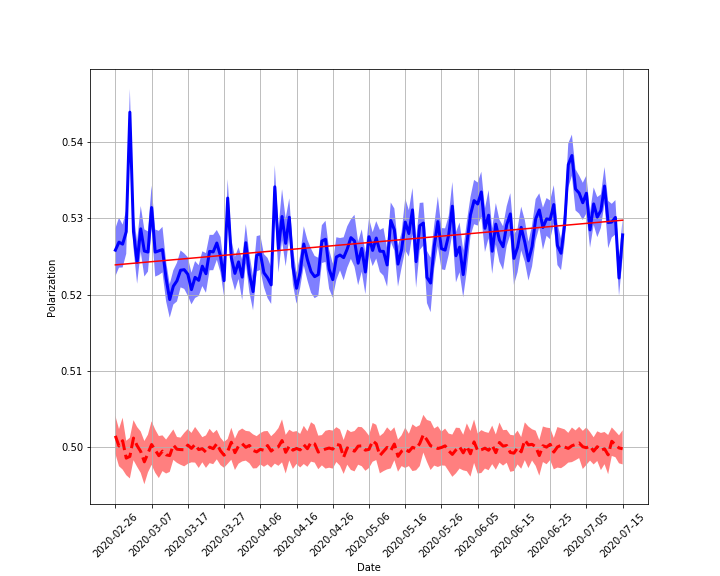
\includegraphics[width=\columnwidth]{figures/polarization_moving_window.png}
		\caption{Polarization estimates from partisanship estimator fitted on a 7-day moving window of vocabulary.}
		\label{fig:polarization_moving_window}
	\end{figure}

	\begin{table}
		\centering
		\begin{tabular}{lrr}
			\toprule
			{} &  constant &     trend \\
			\midrule
			estimate &  0.508833 &  0.000008 \\
			p-value  &  0.000000 &  0.268171 \\
			\bottomrule
		\end{tabular}
	\caption{OLS estimates of trend in daily polarization estimates.}
	\label{tab:polarization_overall_ols}
		
	\end{table}





	\FloatBarrier
	
	\subsection{Topic Modeling}
	
	\begin{figure}[!h]
		\centering
		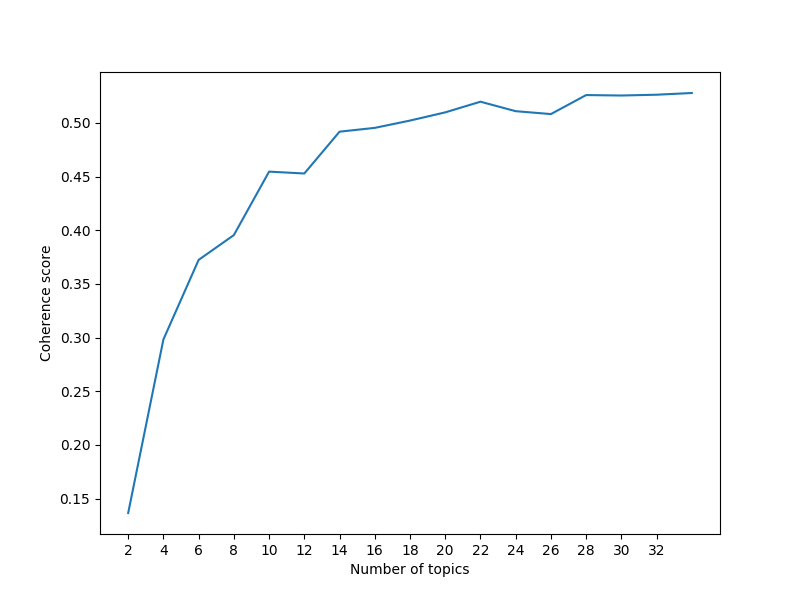
\includegraphics[width=\columnwidth]{figures/coherence_grid.png}
		\caption{Coherence scores for the LDA grid search. Coherence was maximized at 28 topics.}
		\label{fig:coherence_grid}
	\end{figure}


	\begin{figure}[!h]
		\centering
		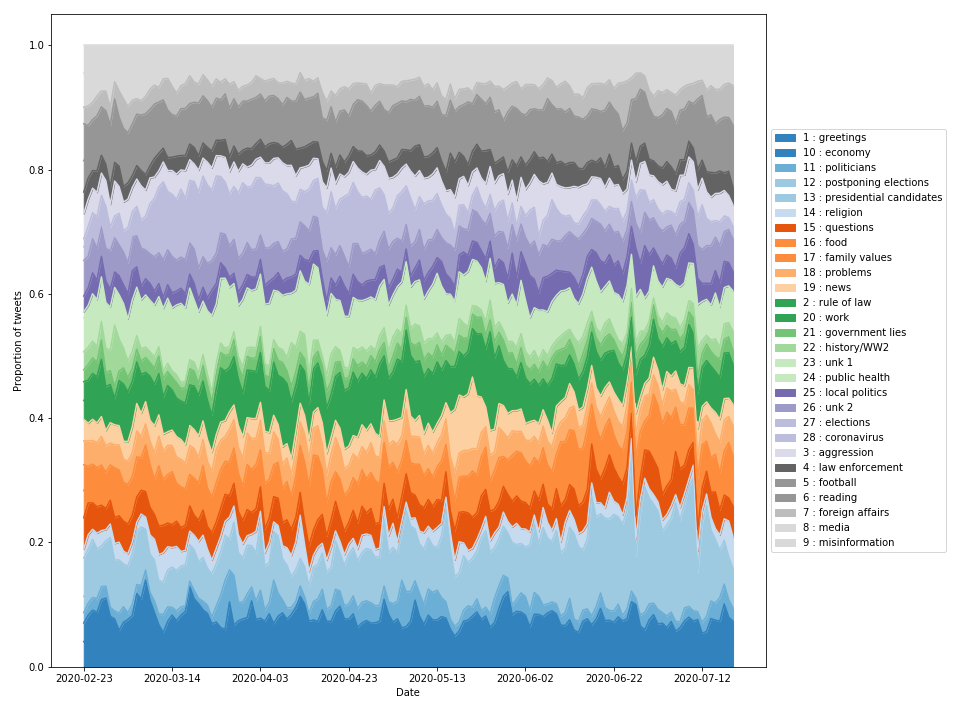
\includegraphics[width=\columnwidth]{figures/temp_dist_all.png}
		\caption{Temporal distribution of all 28 topics identified by the LDA model.}
		\label{fig:topics_time_all }
	\end{figure}

	\FloatBarrier
	
	\clearpage
	
	\subsection{Topic Polarization}
	
	\begin{figure}[!h]
		\centering
		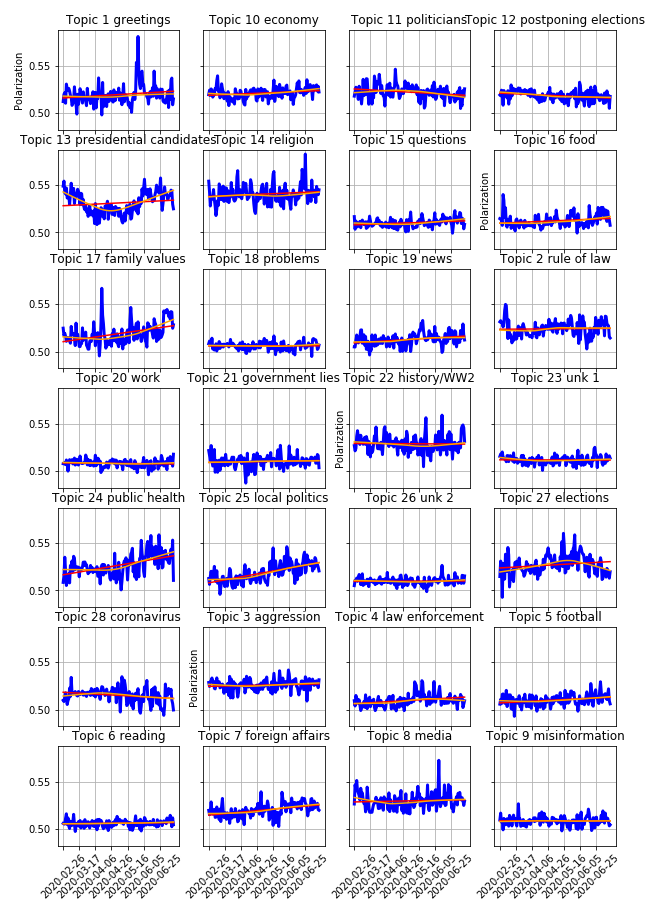
\includegraphics[width=0.8\columnwidth]{figures/polarization_topics_all.png}
		\caption{Polarization estimates for all 28 topics identified by the LDA model.}
		\label{fig:polarization_topics_all}
	\end{figure}

	\clearpage

	\begin{figure}[!h]
		\centering
		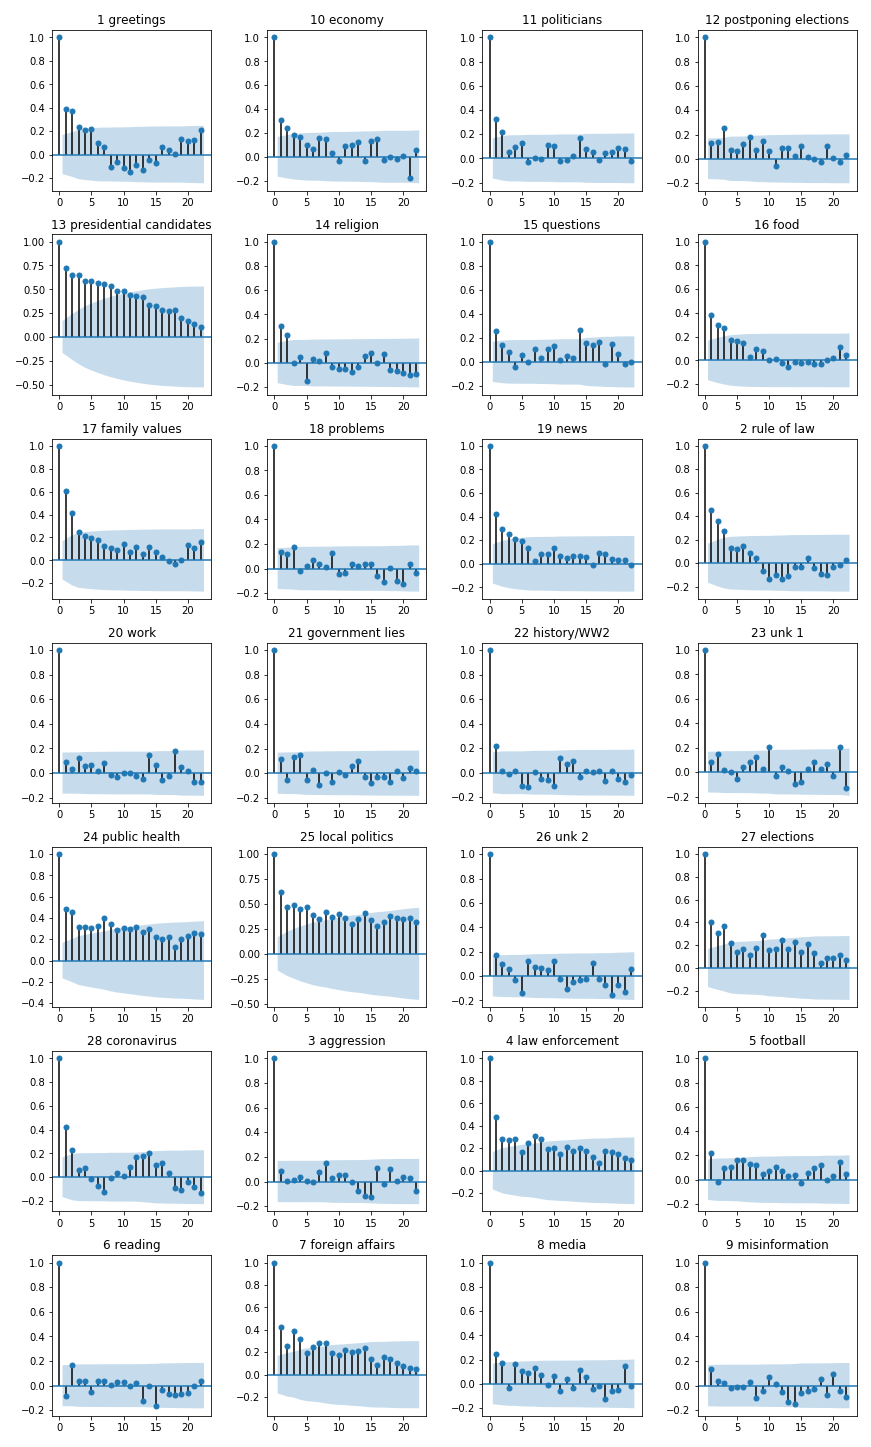
\includegraphics[width=0.8\columnwidth]{figures/topics_autocorrelation.png}
		\caption{Autocorrelation function plot for the daily polarization estimates within each topic.}
		\label{fig:autocorrelation_topics}
	\end{figure}

	\clearpage



	\begin{figure}[!h]
		\centering
		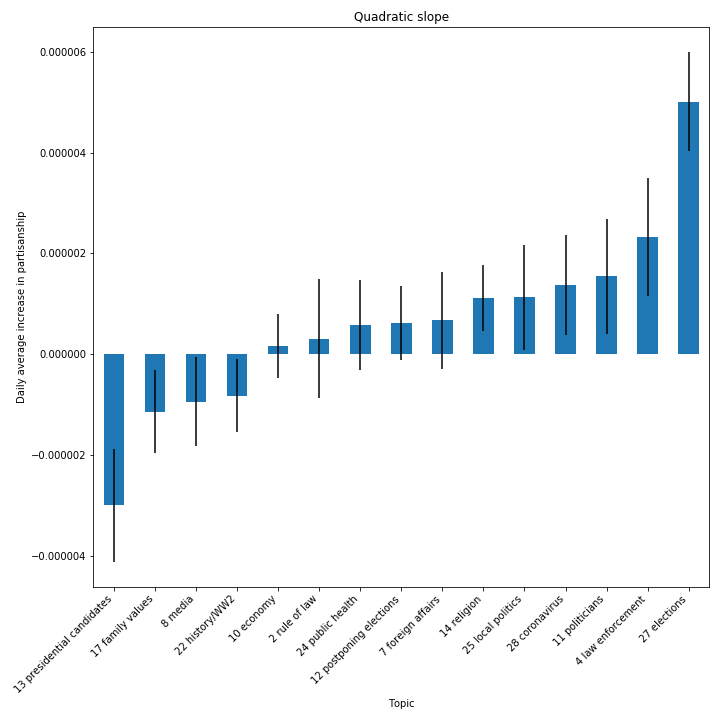
\includegraphics[width=\columnwidth]{figures/partisanship_topics_coef_quadratic.png}
		\caption{Quadratic model coefficients for selected topics. P-value of 0.0 refers to p < .0001.}
		\label{fig:partisanship_topics_coef_quadratic}
	\end{figure}

\clearpage

\begin{longtable}{lrrrr}
	\toprule
	 & \multicolumn{2}{c}{constant} & \multicolumn{2}{c}{slope} \\
	{} &     point & p-value &         point &  p-value \\
	topic                      &           &         &               &          \\
	\midrule
	1 greetings                &  0.515911 &     0.0 &  5.175950e-05 &  0.02039 \\
	10 economy                 &  0.518711 &     0.0 &  3.582105e-05 &  0.00377 \\
	11 politicians             &  0.525369 &     0.0 & -4.825511e-05 &  0.00197 \\
	12 postponing elections    &  0.520982 &     0.0 & -3.747630e-05 &  0.00124 \\
	13 presidential candidates &  0.528101 &     0.0 &  4.248237e-05 &  0.07109 \\
	14 religion                &  0.537868 &     0.0 &  3.685980e-05 &  0.08384 \\
	15 questions               &  0.507954 &     0.0 &  3.061105e-05 &  0.00113 \\
	16 food                    &  0.509692 &     0.0 &  3.685185e-05 &  0.00915 \\
	17 family values           &  0.510574 &     0.0 &  1.232232e-04 &  0.00000 \\
	18 problems                &  0.506099 &     0.0 &  9.125505e-07 &  0.91459 \\
	19 news                    &  0.509364 &     0.0 &  5.157463e-05 &  0.00023 \\
	2 rule of law              &  0.523653 &     0.0 &  6.928925e-06 &  0.69083 \\
	20 work                    &  0.508562 &     0.0 & -7.704487e-06 &  0.35707 \\
	21 government lies         &  0.509025 &     0.0 &  1.488777e-05 &  0.27321 \\
	22 history/WW2             &  0.529152 &     0.0 & -5.373770e-06 &  0.77852 \\
	23 unk 1                   &  0.511824 &     0.0 & -1.944876e-06 &  0.83185 \\
	24 public health           &  0.516393 &     0.0 &  1.465398e-04 &  0.00000 \\
	25 local politics          &  0.507916 &     0.0 &  1.561284e-04 &  0.00000 \\
	26 unk 2                   &  0.509522 &     0.0 &  2.933359e-06 &  0.72967 \\
	27 elections               &  0.523618 &     0.0 &  4.870395e-05 &  0.02822 \\
	28 coronavirus             &  0.518387 &     0.0 & -4.754173e-05 &  0.00355 \\
	3 aggression               &  0.524650 &     0.0 &  1.844353e-05 &  0.13286 \\
	4 law enforcement          &  0.506322 &     0.0 &  5.056352e-05 &  0.00017 \\
	5 football                 &  0.507160 &     0.0 &  4.384077e-05 &  0.00038 \\
	6 reading                  &  0.505480 &     0.0 &  9.379985e-06 &  0.21922 \\
	7 foreign affairs          &  0.514644 &     0.0 &  7.850613e-05 &  0.00000 \\
	8 media                    &  0.528559 &     0.0 &  1.646601e-05 &  0.37033 \\
	9 misinformation           &  0.508644 &     0.0 & -7.282659e-07 &  0.94302 \\
	\bottomrule
\caption{OLS estimates of linear trend in partisanship by topic. P-value of 0.0 refers to p < .0001.}
\label{tab:polarization_topics_ols}
\end{longtable}

\clearpage


\begin{longtable}{lrrrrrr}
	\toprule
	 & \multicolumn{2}{c}{constant} & \multicolumn{2}{c}{linear slope} & \multicolumn{2}{c}{quadratic slope} \\
	{} &     point & p-value &        point &  p-value &           point &  p-value \\
	topic                      &           &         &              &          &                 &          \\
	\midrule
	1 greetings                &  0.515493 &     0.0 &     0.000070 &  0.42600 &   -1.347895e-07 &  0.82858 \\
	10 economy                 &  0.522183 &     0.0 &    -0.000117 &  0.01281 &    1.117944e-06 &  0.00088 \\
	11 politicians             &  0.521849 &     0.0 &     0.000107 &  0.07383 &   -1.133341e-06 &  0.00780 \\
	12 postponing elections    &  0.521489 &     0.0 &    -0.000060 &  0.18810 &    1.634077e-07 &  0.61005 \\
	13 presidential candidates &  0.543643 &     0.0 &    -0.000643 &  0.00000 &    5.004778e-06 &  0.00000 \\
	14 religion                &  0.538832 &     0.0 &    -0.000006 &  0.94630 &    3.105788e-07 &  0.60293 \\
	15 questions               &  0.510006 &     0.0 &    -0.000060 &  0.09659 &    6.606927e-07 &  0.01001 \\
	16 food                    &  0.513999 &     0.0 &    -0.000153 &  0.00446 &    1.386848e-06 &  0.00030 \\
	17 family values           &  0.517798 &     0.0 &    -0.000195 &  0.02048 &    2.326126e-06 &  0.00012 \\
	18 problems                &  0.507390 &     0.0 &    -0.000056 &  0.09640 &    4.159132e-07 &  0.08100 \\
	19 news                    &  0.509431 &     0.0 &     0.000049 &  0.37190 &    2.161955e-08 &  0.95511 \\
	2 rule of law              &  0.525755 &     0.0 &    -0.000086 &  0.21463 &    6.770221e-07 &  0.16613 \\
	20 work                    &  0.509963 &     0.0 &    -0.000069 &  0.03591 &    4.509882e-07 &  0.05362 \\
	21 government lies         &  0.510165 &     0.0 &    -0.000035 &  0.51122 &    3.672418e-07 &  0.33546 \\
	22 history/WW2             &  0.532666 &     0.0 &    -0.000160 &  0.03372 &    1.131816e-06 &  0.03395 \\
	23 unk 1                   &  0.514415 &     0.0 &    -0.000116 &  0.00116 &    8.342791e-07 &  0.00097 \\
	24 public health           &  0.521202 &     0.0 &    -0.000066 &  0.42418 &    1.548809e-06 &  0.00835 \\
	25 local politics          &  0.509732 &     0.0 &     0.000076 &  0.23339 &    5.845878e-07 &  0.19489 \\
	26 unk 2                   &  0.511221 &     0.0 &    -0.000072 &  0.03137 &    5.471880e-07 &  0.02081 \\
	27 elections               &  0.514322 &     0.0 &     0.000459 &  0.00000 &   -2.993538e-06 &  0.00000 \\
	28 coronavirus             &  0.515478 &     0.0 &     0.000081 &  0.20101 &   -9.367261e-07 &  0.03679 \\
	3 aggression               &  0.525832 &     0.0 &    -0.000034 &  0.48769 &    3.805949e-07 &  0.26787 \\
	4 law enforcement          &  0.503783 &     0.0 &     0.000163 &  0.00189 &   -8.176322e-07 &  0.02564 \\
	5 football                 &  0.509435 &     0.0 &    -0.000057 &  0.23312 &    7.324538e-07 &  0.02967 \\
	6 reading                  &  0.506666 &     0.0 &    -0.000043 &  0.15408 &    3.817794e-07 &  0.07336 \\
	7 foreign affairs          &  0.516561 &     0.0 &    -0.000006 &  0.90765 &    6.176227e-07 &  0.09854 \\
	8 media                    &  0.532829 &     0.0 &    -0.000172 &  0.01696 &    1.375071e-06 &  0.00703 \\
	9 misinformation           &  0.508816 &     0.0 &    -0.000008 &  0.83811 &    5.527705e-08 &  0.84728 \\
	\bottomrule
	\caption{Estimates of quadratic trend in polarization within topics.}
	\label{tab:polarization_topics_ols_quadratic}
\end{longtable}



	\FloatBarrier
	
	\clearpage
	
	\subsection{Phrases}
	
	
	\begin{otherlanguage}{polish}
			
			\begin{longtable}{p{2cm}p{2cm}p{5cm}p{5cm}}
				

				\toprule
				topic number &              topic label &                                                                                               opposition phrases &                                                                                                      government phrases \\
				\midrule
				0 &                 multiple &                            tvpis, sasin, suweren, pisowski, adrian, pisowiec, jarek, dudy, morawiecki, kaczyński &                niezalezny pl, dubler, wtylewizja, niezalezny, lewacki, wieszwiecej, lewactwo, wieszwięcy, nitras, budka \\
				1 &                greetings &               cześć, mówić, miły wieczór, popołudnie, trzymać kciuk, kciuk, spokojny dzień, wieczór, pogoda, sen &                 bóg, prawy, duda, pozdrawiać serdecznie, kobieta, dobry spokojny, polska, witać, serdecznie, obserwować \\
				2 &              rule of law &                                pisowski, kaczyński, pis, ziobro, duda, podstawa prawny, krs, równy, tryb, partia &                                  kasta, reforma, gersdorf, opozycja, tsue, wsec, koniec, nadzwyczajny, polak, prezes sn \\
				3 &               aggression &                             pisowski, pis, kaczyński, sort, propaganda, zdradziecki, duda, władza, dziad, kłamca &                                              lewacki, rudy, tw, lewactwo, tęczowy, sb, won, czerwony, trzaskowski, tusk \\
				4 &          law enforcement &                                               mgła, cień, ostry, duda, pis, władza, kraj, policjant, czuć, prawo &                       opozycja, świat, trzaskowski, koronawirus, polak, stawać, niektóry, stosować, podobny, zachowanie \\
				5 &                 football &                                  jarek, pis, musieć, początek, akurat, zaczynać, myśleć, dopiero, raczej, koniec &                                         piłkarz, kibic, szambo, polski, piłka, nadawać, polska, pierwszy, chodzić, klub \\
				6 &                  reading &                               pis, duda, głosować, przekonać, prawy strona, ok, wybory, raz nie, połowa, ostatni &                                   dama, ban, opozycja, obserwować, tweet, nie potrafić, polska, polak, czytać, potrafić \\
				7 &          foreign affairs &               wspólnota, pis, morawiecki, białoruś, unia europejski, trump, unia, amerykanin, mieszkać, otworzyć &              niezalezny pl, niezalezny, defenka, berlin, opozycja, tusk, brukseli, niemiecki, bezpieczeństwo, hiszpania \\
				8 &                    media &                                 wypad, pi, pis, afera, publiczny, silni razem, propaganda, silni, tvp, kaczyński &                                           gw, nitras, sok burak, burak, budka, sok, platform, fake news, lis, platforma \\
				9 &           misinformation &                                  pis, duda, tvp, brać udział, udział, przekaz, wybory, wyraz, nie brać, kontekst &                          trzaskowski, opozycja, manipulacja, źródło, polak, medium, świat, szanowny, dokładnie, artykuł \\
				10 &                  economy &                             pisowski, szumowski, kaczyński, dudy, pi, morawiecki, węgla, tvp, pis, wolny podatek &                                      ofe, psl, tusk, trzaskowski, warszawa, pit, wiek emerytalny, emerytalny, wiek, gaz \\
				11 &              politicians &                         kaczyński, wyborczy, lewica, witek, poprawka, głosowanie, prawo, odrzucić, pis, podpisać &       totalny opozycja, totalny, grodzki, konfederacja, bosak, marszałek grodzki, sld, obywatelski, trzaskowski, polska \\
				12 &     postponing elections &                                   pisowski, utrzymać, pi, kaczyński, pis, morawiecki, trup, duda, rząd pis, ręka &                              psl, totalny, tusk, opozycja, chaos, trzaskowski, polski, przejąć, chodzić, stan wyjątkowy \\
				13 &  presidential candidates &                    padz pałac, padz, prezydent trzaskowski, pałac, wkk, silny, biedron, kaczyński, lewica, wejść &  dubler, duda prezydent, duda andrzej, wieszwięcy, prezydent andrzej, sprawa, polski, prezydent duda, plan, duda wybory \\
				14 &                 religion &                                religia, boski, biskup, katolicki, cud, ksiądz, katolik, chodzić, kościół, polski &                        szczęść bóg, szczęść, bóg zapłać, miłosierdzia, zapłać, św jan, msza św, św, paweł ii, dziękować \\
				15 &                questions &                    kaczyński, duda, obcy, prezes, pis, tvp, prasowy, konferencja, konferencja prasowy, angielski &        trzaskowski, nie interesować, interesować, polak, krótko, załatwić, opozycja, wiedzieć wiedzieć, poseł, szczerze \\
				16 &                     food &                                              pis, ryż, wino, kot, kawa, prosić, uwielbiać, ciepły, jutro, koniec &                                           polski, biały, tyle, kupować, polska, wódka, żona, sklep, wziąć, siedzieć dom \\
				17 &            family values &                                   duda, pedofil, pis, ofiara, przemoc, prezydent, osoba, polski, wobec, edukacja &                                    aborcja, trzaskowski, ideologia, mężczyzna, czarny, szkół, matka, lgbt, życie, stary \\
				18 &                 problems &                              pis, władza, przygotować, duda, pytanie, obawiać, sukces, głosować, wciąż, kampania &                                     powrót, opozycja, dom, wirus, odpowiedni, szybki, prosić, korzystać, polska, szybko \\
				19 &                     news &                                    pis, fb, wiadomość, marek, trzaskowski, znaleźć, piosenka, włączyć, duda, tvp &                                       tvrepublik, zostańwdom, tube, red, sztuka, dr, zachęcać, godz, polska, informacja \\
				20 &                     work &                                  ostatni rok, pis, tracić, niedługo, firma, duda, ostatni, minuta, państwo, kraj &                                       bóg, opozycja, dać spokój, trudny, spokój, minąć, matura, ciężki, zakład, martwić \\
				21 &          government lies &                                                   pis, duda, kraść, kasa, mafia, nikt, chyba, kłamać, wybory, sa &                                               polak, trzaskowski, polska, tyle, chcieć, rzad, ktor, czas, reszta, dawać \\
				22 &              history/WW2 &                                  pis, smoleński, kaczyński, katastrofa, grób, dobry, móc, duda, człowiek, siebie &                                      ub, sowiecki, komunistyczny, śp, stanisław, niemiec, jan, ps, komunista, niemiecki \\
				23 &                    unk 1 &                                           lud, kaczyński, ciemny, duda, pis, prezes, strach, ból, mieścić, śmiać &                                          opozycja, kupa, dzban, trzaskowski, kobieta, kamień, pisać, nosić, nos, rzucać \\
				24 &            public health &  pis, test, wybory, ministerstwo zdrowie, duda, przygotować, środek ochrona, ochrona zdrowie, ministerstwo, brak &                                     operacja, owsiak, uratować, dziękować, błagać, rt, tys, wesprzeć, pomagać, wspierać \\
				25 &           local politics &                            elektryczny, pis, region, zwierzę, wrocław, susza, auto, szczecin, klimat, mieszkanie &                                   ratusz, czajka, strefa, czytać, warszawski, wisła, stolica, gdańsk, warszawa, wiślany \\
				26 &                    unk 2 &                                         pisowski, kaczyński, duda, pis, władza, kraj, tvp, naród, moralny, prawo &                                  opozycja, wypisywać, bóg, trzaskowski, zachowywać, debil, kobieta, wpis, poziom, polak \\
				27 &                elections &                  sasin, sasina, kaczyński, wydrukować, jacek, drukować, organizować, pis, karta wyborczy, pakiet &                     koperta, opozycja, obietnica, zbierać podpis, lokal, lokal wyborczy, odbyć, zbierać, termin, plakat \\
				28 &              coronavirus &                          pis, pi, duda, liczba test, wybory, szumowski, sanepid, robić test, testować, wykonywać &        wieszwięcy, woj, szwecja, hiszpania, koronawirus sars, koronawirus covid, szczepionek, grypa, wuhan, coronavirus \\
				
				\bottomrule
				
				\caption{Full list of top 10 party-specific lemmas in Polish.}
				\label{tab:party_phrases_pol_full}

		\end{longtable}
		

\clearpage

\begin{longtable}{p{2cm}p{2cm}p{5cm}p{5cm}}
	
	
	\toprule
	topic number &              topic label &                                                                                                                                                                opposition phrases &                                                                                                                                                                               government phrases \\
	\midrule
	0 &                 multiple &  tvpis [mock name for state TV], sasin [Interior Minister], sovereign, pisowski [governing party], adrian, writer, jarek [Kaczynski], bagpipe, Morawiecki, Kaczynski [PiS leader] &                                                              independent pl, double, recession, independent, leftist, more, leftism, knowmore, nitras [opposition MP], Budka [opposition leader] \\
	1 &                greetings &                                                                                Hello, speak, nice evening, afternoon, hold your thumb, thumb, a calm day, evening, weather, dream &                                                                                      God, right, Duda [incumbent president], greet cordially, woman, good calm, Poland, greet, heartily, observe \\
	2 &              rule of law &                                 pisowski [governing party], Kaczynski [PiS leader], PiS [governing party], ribs, Duda [incumbent president], legal basis, krs, equal, mode, party &                                                                                                     caste, reform, gersdorf, opposition, tsue, insert, end, extraordinary, Pole, president of sn \\
	3 &               aggression &                pisowski [governing party], PiS [governing party], Kaczynski [PiS leader], sort, propaganda, treacherous, Duda [incumbent president], authority, grandfather, liar &                                                                        leftist, ore, tw, leftism, rainbow, Sat, won, red, Trzaskowski [opposition presidential candidate, Mayor of Warsaw], tusk \\
	4 &          law enforcement &                                                            fog, shadow, sharp, Duda [incumbent president], PiS [governing party], authority, country, police officer, feel, right &                                                     opposition, world, Trzaskowski [opposition presidential candidate, Mayor of Warsaw], coronavirus, Pole, to stop, one, use, similar, behavior \\
	5 &                 football &                                                                               jarek [Kaczynski], PiS [governing party], must, beginning, exactly, start, think, only, rather, end &                                                                                                                 footballer, waist, septic tank, Polish, ball, broadcast, Poland, first, go, club \\
	6 &                  reading &                                                              PiS [governing party], Duda [incumbent president], vote, convince, right side, okay, elections, once not, half, last &                                                                                                                      lady, ban, opposition, observe, tweet, Can not, Poland, Pole, read, be able \\
	7 &          foreign affairs &                                                                         community, PiS [governing party], Morawiecki, Belarus, European union, trump, union, American, live, open &                                                                                                independent pl, independent, defenka, Berlin, opposition, tusk, Brussels, German, security, Spain \\
	8 &                    media &                                                            excursion, pi, PiS [governing party], affair, public, strong together, propaganda, strong, tvp, Kaczynski [PiS leader] &  gw [liberal newspaper], nitras [opposition MP], sok burak [online opposition platform], burak, Budka [opposition leader], sok [online opposition platform], platforms, fake news, Nov, platform \\
	9 &           misinformation &                                               PiS [governing party], Duda [incumbent president], tvp, participate, participation, transfer, elections, word, do not take, context &                                             Trzaskowski [opposition presidential candidate, Mayor of Warsaw], opposition, manipulation, source, Pole, medium, world, honorable, exactly, article \\
	10 &                  economy &                              pisowski [governing party], Szumowski [Health Minister], Kaczynski [PiS leader], bagpipe, pi, Morawiecki, coal, tvp, PiS [governing party], free tax &                                                              ofe, psl, tusk, Trzaskowski [opposition presidential candidate, Mayor of Warsaw], Warsaw, pit, retirement age, retirement, age, gas \\
	11 &              politicians &                                          Kaczynski [PiS leader], electoral, left, Witek [Speaker of the Parliament], correction, vote, right, reject, PiS [governing party], sign &                                      total opposition, total, township, confederation, Bosak, town marshal, sld, civil, Trzaskowski [opposition presidential candidate, Mayor of Warsaw], Poland \\
	12 &     postponing elections &   pisowski [governing party], maintain, pi, Kaczynski [PiS leader], PiS [governing party], Morawiecki, corpse, Duda [incumbent president], government pis [governing party], hand &                                                 psl, total, tusk, opposition, chaos, Trzaskowski [opposition presidential candidate, Mayor of Warsaw], Polish, take over, go, state of emergency \\
	13 &  presidential candidates &       PAD out of palace, padz, President of Trzaskowski [opposition presidential candidate, Mayor of Warsaw], palace, wkk, powerful, Biedron, Kaczynski [PiS leader], left, enter &         double, Duda president [incumbent president], duda andrzej [incumbent president], knowmore, president andrzej, case, Polish, President Duda [incumbent president], plan, booty elections \\
	14 &                 religion &                                                                                                 religion, divine, bishop, Catholic, miracle, priest, Catholic, go, church, Polish &                                                                                                              bless god, happiness, God bless you, mercy, pay, St. John, mass, st, Paul ii, thank \\
	15 &                questions &                          Kaczynski [PiS leader], Duda [incumbent president], foreign, president, PiS [governing party], tvp, press release, conference, press conference, English &                                         Trzaskowski [opposition presidential candidate, Mayor of Warsaw], not interested, interest, Pole, short, arrange, opposition, know know, envoy, honestly \\
	16 &                     food &                                                                                                   PiS [governing party], rice, wine, cat, coffee, ask, adore, warm, tomorrow, end &                                                                                                                           Polish, white, so much, buy, Poland, vodka, wife, shop, take, sit home \\
	17 &            family values &                                                          Duda [incumbent president], pedophile, PiS [governing party], victim, violence, President, person, Polish, to, education &                                                               abortion, Trzaskowski [opposition presidential candidate, Mayor of Warsaw], ideology, man, black, schools, mother, lgbt, life, old \\
	18 &                 problems &                                                          PiS [governing party], authority, prepare, Duda [incumbent president], question, to fear, success, vote, still, campaign &                                                                                                                         return, opposition, House, virus, suitable, fast, ask, use, Poland, fast \\
	19 &                     news &               PiS [governing party], fb, message, brands, Trzaskowski [opposition presidential candidate, Mayor of Warsaw], found, song, turn on, Duda [incumbent president], tvp &                                                                                                                     tvrepublik, stay home, tube, ed, art, dr, encourage, at, Poland, information \\
	20 &                     work &                                                               last year, PiS [governing party], to lose, soon, business, Duda [incumbent president], last, minute, state, country &                                                                                                                  God, opposition, give a break, hard, calm, pass, matura exam, heavy, bet, worry \\
	21 &          government lies &                                                              PiS [governing party], Duda [incumbent president], steal, cash register, mafia, no one, I guess, lie, elections, are &                                                            Pole, Trzaskowski [opposition presidential candidate, Mayor of Warsaw], Poland, so much, want, government, which, time, rest, to give \\
	22 &              history/WW2 &  PiS [governing party], Smolensk [location of 2010 presidential plane crash], Kaczynski [PiS leader], a disaster, grave, good, power, Duda [incumbent president], man, each other &                                                                                                                    last, soviet, Communist, late, stanislaw, German, john, ps, Communist, German \\
	23 &                    unk 1 &                                                     people, Kaczynski [PiS leader], dark, Duda [incumbent president], PiS [governing party], president, fear, pain, fit, to laugh &                                                              opposition, heap, pitcher, Trzaskowski [opposition presidential candidate, Mayor of Warsaw], woman, stone, write, wear, nose, throw \\
	24 &            public health &                               PiS [governing party], test, elections, health ministry, Duda [incumbent president], prepare, protection measure, health protection, ministry, lack &                                                                                           operation, Owsiak [liberal health activist], save, thank, beg, rt, thousand, to support, help, support \\
	25 &           local politics &                                                                                   electric, PiS [governing party], region, animal, Wroclaw, drought, car, Szczecin, climate, flat &                                                         town hall, Czajka [malfunctioning sewage treatment plant in Warsaw], zone, read, Warsaw, Vistula, capital, gdańsk, Warsaw, Vistula river \\
	26 &                    unk 2 &                              pisowski [governing party], Kaczynski [PiS leader], Duda [incumbent president], PiS [governing party], authority, country, tvp, nation, moral, right &                                                           opposition, unsubscribe, God, Trzaskowski [opposition presidential candidate, Mayor of Warsaw], keep, idiot, woman, entry, level, Pole \\
	27 &                elections &                          sasin [Interior Minister], sasina [Interior Minister], Kaczynski [PiS leader], print, Jack, print, organize, PiS [governing party], voting card, package &                                                                                  envelope, opposition, promise, collect a signature, station, polling station, take place, collect, term, poster \\
	28 &              coronavirus &         PiS [governing party], pi, Duda [incumbent president], number of test, elections, Szumowski [Health Minister], sanepid [CDC equivalent], do the test, to test, to perform &                                                                                            knowmore, voiv, Sweden, Spain, coronavirus sars, covid coronavirus, vaccines, flu, wuhan, coronavirus \\
	\bottomrule
	
		\caption{Full list of top 10 party-specific lemmas in English.}
		\label{tab:party_phrases_en_full}
	\end{longtable}
	
	
\end{otherlanguage}
	
\end{document}